\documentclass[ignorenonframetext,]{beamer}
\PassOptionsToPackage{hyphens}{url}
\usepackage{pgfpages}
\setbeamertemplate{caption}[numbered]
\setbeamertemplate{caption label separator}{: }
\setbeamercolor{caption name}{fg=normal text.fg}
\beamertemplatenavigationsymbolsempty
\usepackage{lmodern}
\usepackage{amssymb,amsmath}
\usepackage{ifxetex,ifluatex}
\usepackage[T1]{fontenc}
\usepackage[utf8]{inputenc}
\usepackage{textcomp} % provides euro and other symbols
\usetheme[]{theme}
%\IfFileExists{microtype.sty}{%
%\usepackage[]{microtype}
%\UseMicrotypeSet[protrusion]{basicmath} % disable protrusion for tt fonts
%}{}
\usepackage{multicol}
\usepackage{tikz}
\usetikzlibrary{shadows,arrows,positioning}
%\setlength{\parindent}{0pt}
%\setlength{\parskip}{6pt plus 2pt minus 1pt}
\urlstyle{same}  % don't use monospace font for urls
\makeatletter
\def\maxwidth{\ifdim\Gin@nat@width>\linewidth\linewidth\else\Gin@nat@width\fi}
\def\maxheight{\ifdim\Gin@nat@height>\textheight\textheight\else\Gin@nat@height\fi}
\makeatother
% Scale images if necessary, so that they will not overflow the page
% margins by default, and it is still possible to overwrite the defaults
% using explicit options in \includegraphics[width, height, ...]{}
\setkeys{Gin}{width=\maxwidth,height=\maxheight,keepaspectratio}
% Prevent slide breaks in the middle of a paragraph:
%\widowpenalties 1 10000
%\raggedbottom
\setbeamertemplate{section page}{
\begin{beamercolorbox}[sep=12pt,center]{part title}
  \usebeamerfont{section title}\insertsection\par
\end{beamercolorbox}
}
\setlength{\emergencystretch}{3em}  % prevent overfull lines
\setcounter{secnumdepth}{0}

\title{Les réseaux de neurones}
\author{Fabien Bernier, Elouen Ginat \& Simon Thoby}
\date{Juin 2018}

\begin{document}
\section*{Présentation}
\frame{\titlepage}

\begin{frame}{Sommaire}
\tableofcontents
\end{frame}

\section{Les réseaux de neurones}
\frame{\sectionpage}
\begin{frame}{Structure générale}
	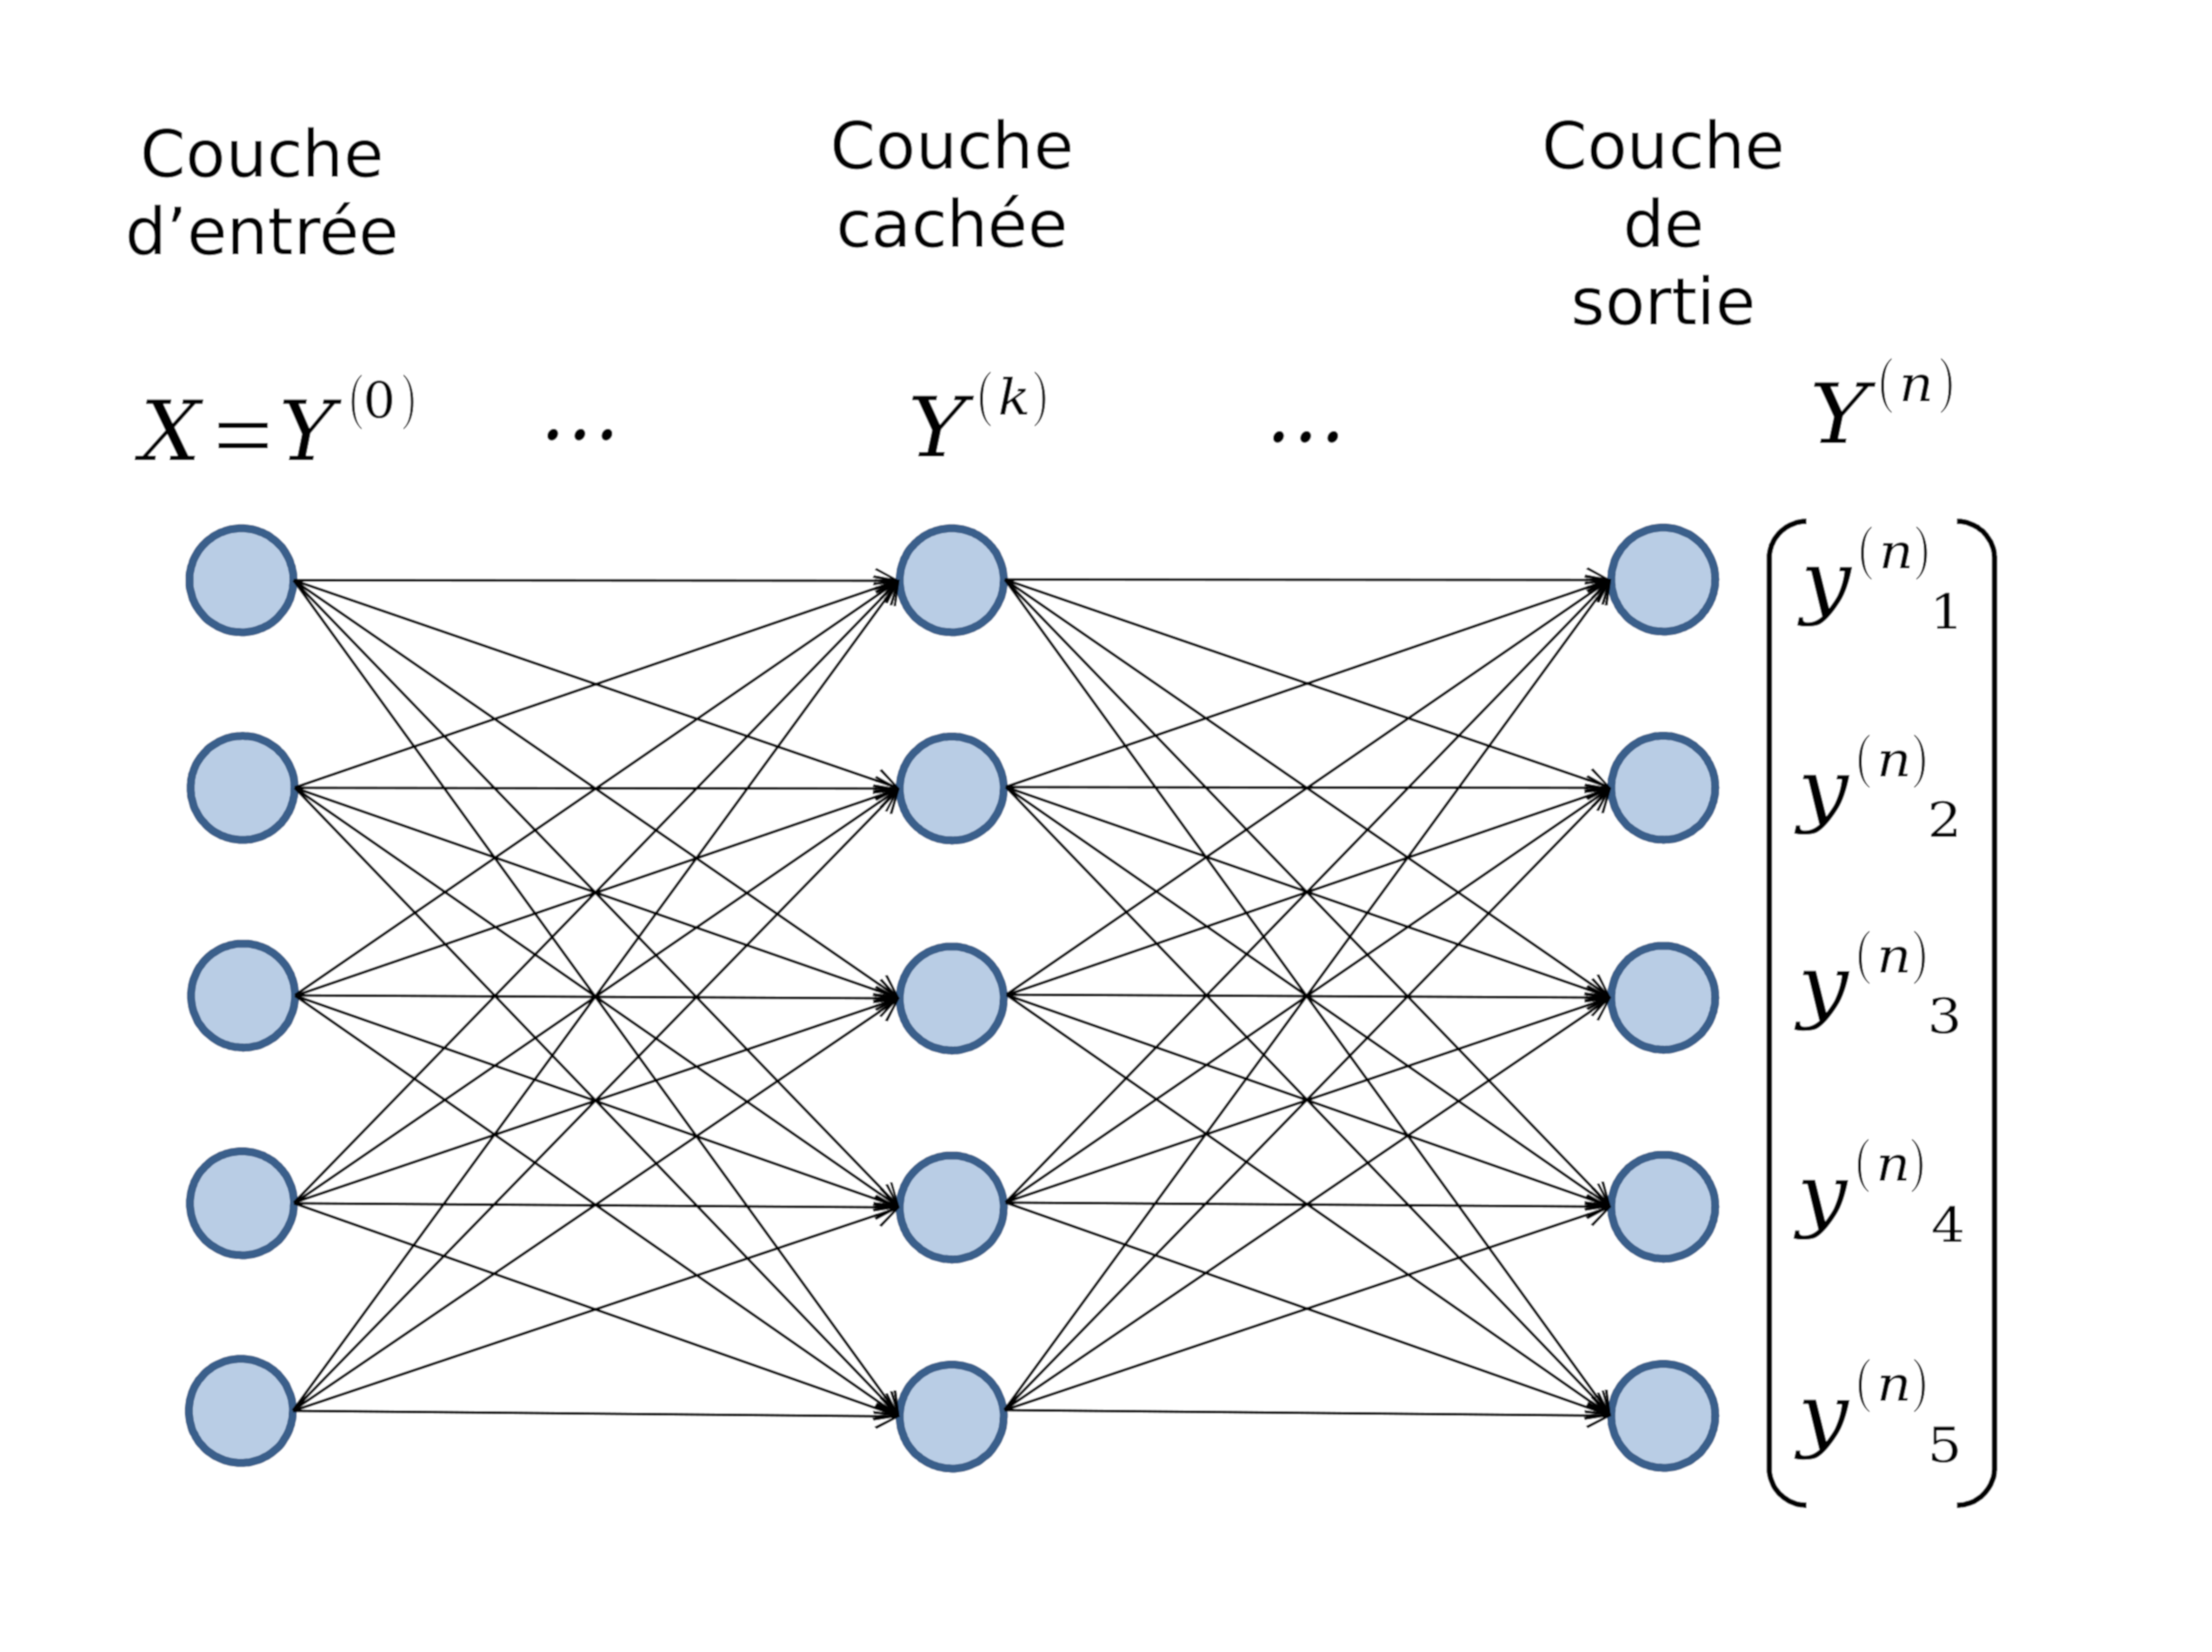
\includegraphics{net-without-train.png}
\end{frame}

\begin{frame}{Fonctionnement du réseau}
    - Accepte un vecteur en entrée : que l'on considére comme la première couche, notée $ Y^0 $ \\
    - Pour chaque couche, on génére un nouveau vecteur à partir de la couche précédente en effectuant une somme pondérée des valeurs de la couche précédente : \[ Y^n = \tilde\alpha(W^n . Y^{n-1} + B^n) \]
        Avec :
    \begin{itemize}
        \item $ \alpha $ : une fonction (dérivable) qui sert à améliorer l'efficacité du réseau en normalisant les sorties, classiquement $ \alpha : x \mapsto \frac{1}{1+e^{-x}} $
        \item $\tilde\alpha$ : la fonction $\alpha$ appliquée à chacun des élements d'un vecteur.
        \item $ W^n $ : les poids de passage de la couche $ n-1 $ à $ n $
        \item $ B^n $ : les biais de la couche $ n $, qui permettent au réseau d'approximer des fonctions qui ne s'annulent pas quand l'entrée est nulle
    \end{itemize}
    - Retourne un vecteur en sortie : la sortie de la dernière couche, c'est-à-dire $ Y^n $
\end{frame}

\begin{frame}{Fonctionnement du réseau - Suite}
	On dispose pour créer le réseau de deux jeux de données assez conséquent (typiquement plusieurs milliers d'images dans notre cas) : l'un sert à entraîner le réseau et l'autre sert à en tester l'efficacité.
    \begin{align*}
        B^k = \begin{pmatrix} b_1^k \\ b_2^k \\ \vdots \\ b_l^k \end{pmatrix}
        &&&
        Y^k = \begin{pmatrix} y_1^k \\ y_2^k \\ \vdots \\ y_l^k \end{pmatrix}
        \\
        \tilde\alpha : X = \begin{pmatrix}
            x_1 \\
            x_2 \\
            \vdots \\
            x_n
        \end{pmatrix} \mapsto \begin{pmatrix}
            \alpha(x_1) \\
            \alpha(x_2) \\
            \vdots \\
            \alpha(x_n)
        \end{pmatrix} &&&
        W^k = \begin{pmatrix}
            w_{11}^k  & w_{21}^k & \cdots & w_{l1}^k \\
            w_{12}^k  & w_{22}^k & \cdots & w_{l2}^k \\
            \vdots & \vdots & \ddots & \vdots \\
            w_{1l}^k  & w_{2l}^k & \cdots & w_{ll}^k
        \end{pmatrix}
    \end{align*}
\end{frame}

\section{La rétropropagation}
\frame{\sectionpage}
\begin{frame}{Approximation d'une fonction}
	À l'instar du théorème d'approximation d'une fonction continue par un polynôme (Stone-Weierstrass), les réseaux de neurones ont pour but d'approximer une fonction dont on ne connaît généralement pas l'expression. Pour ce faire, on utilise généralement l'algorithme dit de «descente du gradient». Le principe est le suivant : \\
    - Le gradient indique la direction de l'augmentation d'une fonction. \\
    - On peut donc considérer la fonction $E$ qui indique l'«erreur» du réseau, c'est à dire la distance entre les sorties du réseau et les valeurs attendues en sortie. \\
    - Notre but est donc de faire tendre les sorties du réseau vers les valeurs attendues, donc de minimiser cette fonction. \\
\end{frame}

\begin{frame}{Correction des poids et des biais}
    Les données d'entrées ne sont pas des paramètres de notre fonction d'erreur, car on cherche à réduire l'erreur du réseau en modifiant les variables du réseau et non pas l'entrée, cela n'aurait pas de sens : $ E = E(w_{11}^1, w_{12}^n, ..., w_{ll}^n, b_1^1, n_2^1, ..., b_l^n) $.
    Pour ce faire, on dérive l'erreur par rapport aux paramètres de notre réseau (les poids et les biais). \\
    Puis on mets à jour les poids et les biais :
    \[ w_{ij}^{(n)} \longleftarrow w_{ij}^{(n)} - \eta \frac{\partial{E}}{\partial{w_{ij}^{(n)}}} \]
    \[ b_i^{(n)} \longleftarrow b_i^{(n)} - \eta \frac{\partial{E}}{\partial{b_i^{(n)}}} \]
\end{frame}

\begin{frame}{La rétropropagation}
    Les problèmes qui ont longtemps concentrés les efforts de la recherche sur les réseaux de neurones, outre la lourdeur de calcul, tournaient autour de la difficulté à concevoir et entraîner des réseaux multicouches. C'est là que l'algorithme de la rétropropagation appraît : il exploite le \textbf{théorème de dérivation des fonctions composées} pour calculer toutes ces dérivées.\\
    L'algorithme est itératif, travaillant couche par couche, en partant de la dernière couche et en remontant jusqu'à la couche d'entrée du réseau, d'où son nom. \\
    Un exemple assez classique de fonction d'erreur est la distance quadratique entre le vecteur obtenu et le vecteur attendu :
    \[ E = \frac{1}{2} \sum_{i=1}^l (y_i^n-a_i)^2 \]
\end{frame}

\begin{frame}{La rétropropagation - Suite}
    Les calculs sont très simples pour la première couche :
    \begin{flalign*}
        \frac{\partial{E}}{\partial{b_k^n}} &= \frac{\partial{E}}{\partial{y_k^n}} \frac{\partial{y_k^n}}{\partial{b_k^n}} &\\
        \text{Or :}  &&\\
        \frac{\partial{E}}{\partial{y_k^n}} &= y_k^n-a_k &\\
        \frac{\partial{y_k^n}}{\partial{b_k^n}} &= \frac{\partial{(\alpha(\sum_{i=0}^l w_{ik}^n*y_i^{n-1} + b_k^n))}}{\partial{b_k^n}} &\\
        &= \alpha'(\sum_{i=0}^l w_{ik}^n*y_i^{n-1} + b_k^n) &\\
        \text{Donc :} &&\\
        \frac{\partial{E}}{\partial{b_k^n}} &= (y_k^n-a_k)*\alpha'(\sum_{i=0}^l w_{ik}^n*y_i^{n-1} + b_k^n) &
    \end{flalign*}
\end{frame}

\begin{frame}{La rétropropagation - Suite}
    Il en va de même pour les poids:
    \begin{flalign*}
        \frac{\partial{E}}{\partial{w_{ik}^n}} &= \frac{\partial{E}}{\partial{y_k^n}} \frac{\partial{y_k^n}}{\partial{w_{ik}^n}} &\\
        \text{Or :}  &&&&\\
        \frac{\partial{E}}{\partial{y_k^n}} &= y_k^n-a_k &\\
        \frac{\partial{y_k^n}}{\partial{w_{ik}^n}} &= \frac{\partial{(\alpha(\sum_{i=0}^l w_{ik}^n*y_i^{n-1} + b_k^n))}}{\partial{w_{ik}^n}} &\\
        &= y_i^{n-1} * \alpha'(\sum_{i=0}^l w_{ik}^n*y_i^{n-1} + b_k^n) &\\
        \text{Donc :} &&&&\\
        \frac{\partial{E}}{\partial{w_{ik}^n}} &= y_i^{n-1}*(y_k^n-a_k)*\alpha'(\sum_{i=0}^l w_{ik}^n*y_i^{n-1} + b_k^n) &
    \end{flalign*}
\end{frame}
\begin{frame}{La rétropropagation - Suite}
    Les choses se compliquent néanmoins pour les couches précédentes: en effet, la dérivée de l'erreur en fonction du poids ou des biais d'un neurone de la couche $k$ dépend de la dérivée de l'erreur en fonction de tous les neurones de la couche $k+1$ :
    \[ \frac{\partial{E}}{\partial{b_1^k}} = \sum_{i=0}^l \frac{\partial{E}}{\partial{y_i^{k+1}}} \frac{\partial{y_i^{k+1}}}{\partial{b_1^k}} \]
Fort heureusement, on vient de calculer $ \frac{\partial{E}}{\partial{y_i^n}} $ et on peut simplement calculer $ \frac{\partial{y_i^n}}{\partial{b_1^{n-1}}} $. On peut donc mettre à jour les poids et les biais de la couche $n-1$. En appliquant récursivement cette méthode, on peut ainsi actualiser tous les poids et tous les biais du réseau.
\end{frame}

\section{Exemple}
\frame{\sectionpage}
\begin{frame}{Un exemple simple: un porte logique ET à trois entrées}
    \begin{tikzpicture}
    [   cnode/.style={draw=black,fill=####1,minimum width=3mm,circle},
    ]
        \node[cnode=red,label=0:$y_1^2$] (s) at (6,-2) {};
        \foreach \x in {1,...,3} {
            \node[cnode=blue,label=180:$y_\x^1$] (y1-\x) at (0,2-2*\x) {};
            \node[cnode=blue,label=90:$y_\x^2$] (y2-\x) at (3,2-2*\x) {};
            \draw (y2-\x) -- node[above,sloped,pos=0.4] {$w_{\x1}^2$} (s);
        }
        \foreach \x in {1,...,3} {
            \foreach \y in {1,...,3} {
                \draw (y1-\x) -- (y2-\y);
            }
        }
    \end{tikzpicture}
    //TODO: add logical table
\end{frame}

\begin{frame}{Un exemple simple: un porte logique ET à trois entrées}
    $ \forall i \in \{1, 2\}, \forall k \in \{1, 2, 3\} $
    \begin{flalign*}
        \alpha &= id &\\
        y_i^1 &= w_{1i}^1 * y_1^0 + w_{2i}^1 * y_2^0 + w_{3i}^1 * y_3^0 + b_i^1 &\\
        y_1^2 &= w_{11}^2 * y_1^1 + w_{21}^2 * y_2^1 + b_k^2 &\\
        E &= \frac{(y_1^2-a_1)^2}{2} &\\
        \frac{\partial{E}}{\partial{b_1^2}} &= \frac{\partial{E}}{\partial{y_1^2}} &\\
        &= y_1^2-a_1 &\\
        \frac{\partial{E}}{\partial{w_{i1}^2}} &= y_i^1 * (y_1^2-a_1) &
    \end{flalign*}
\end{frame}

\begin{frame}{Un exemple simple: un porte logique ET à trois entrées}
    \begin{flalign*}
        \frac{\partial{E}}{\partial{b_i^1}} &= \frac{\partial{E}}{\partial{y_i^1}} &\\
        &= \frac{\partial{E}}{\partial{y_1^2}} \frac{\partial{y_1^2}}{\partial{b_i^1}} + \frac{\partial{E}}{\partial{y_2^2}} \frac{\partial{y_2^2}}{\partial{b_i^1}} &\\
        &= w_{i1}^2 * (y_1^2-a_1) + w_{i2}^2 * (y_2^2-a_2) &\\
        \frac{\partial{E}}{\partial{w_{ki}^1}} &= \frac{\partial{E}}{\partial{y_1^2}} \frac{\partial{y_1^2}}{\partial{w_{ki}^1}} + \frac{\partial{E}}{\partial{y_2^2}} \frac{\partial{y_2^2}}{\partial{w_{ki}^1}} &\\
        &= y_k^0 * w_{i1}^2 * (y_1^2-a_1) + y_k^0 * w_{i2}^2 * (y_2^2-a_2)
    \end{flalign*}
    //TODO: add diagramm
\end{frame}
%\begin{frame}{}
%
%\[ P^{(k)} = W^{(k)}Y^{(k-1)}+B^{(k)}  \]
%
%\[ \alpha : x \mapsto \frac{1}{1+e^{-x}} \]
%
%\[ Y^{(k)} = \tilde\alpha(P^{(k)}) \]
%
%\[ E = \frac{1}{2} \sum_{i=1}^l (y_i^{(n)}-a_i)^2 \]
%
%\end{frame}
%
%\begin{frame}{}
%
%\[ b_i^{(n)} \longleftarrow b_i^{(n)} - \eta \frac{\partial{E}}{\partial{b_i^{(n)}}} \]
%
%\[ w_{ij}^{(n)} \longleftarrow w_{ij}^{(n)} - \eta \frac{\partial{E}}{\partial{w_{ij}^{(n)}}} \]
%
%\[ \frac{\partial{E}}{\partial{b_i^{(n)}}} = \frac{\partial{E}}{\partial{p_i^{(n)}}} \frac{\partial{p_i^{(n)}}}{\partial{b_i^{(n)}}} \]
%
%\[ p_i^{(n)} = \sum_{j=1}^l w_{ij}^{(n)} y_j^{(n-1)} + b_i^{(n)} \]
%
%\end{frame}
%
%\begin{frame}{}
%
%\[ \delta_i^{(n)} = \frac{\partial{E}}{\partial{p_i^{(n)}}} = \frac{\partial{E}}{\partial{b_i^{(n)}}} \]
%
%\[ \delta_i^{(n)} = \frac{\partial{E}}{\partial{p_i^{(n)}}} = \frac{\partial{E}}{\partial{y_i^{(n)}}} \frac{\partial{y_i^{(n)}}}{\partial{p_i^{(n)}}} \]
%
%\[ y_i^{(n)} = \alpha(p_i^{(n)}) \implies \frac{\partial{y_i^{(n)}}}{\partial{p_i^{(n)}}} = \alpha'(p_i^{(n)}) \]
%
%\[ E = \frac{1}{2} \sum_{i=1}^l (y_i^{(n)}-a_i)^2 \implies \frac{\partial{E}}{\partial{y_i^{(n)}}} = y_i^{(n)} - a_i \]
%
%\end{frame}
%
%\begin{frame}{}
%
%\[ \delta_i^{(n)} = \alpha'(p_i^{(n)}) (y_i^{(n)} - a_i) \]
%
%\[ \frac{\partial{E}}{\partial{w_{ij}^{(n)}}} = \frac{\partial{E}}{\partial{p_i^{(n)}}} \frac{\partial{p_i^{(n)}}}{\partial{w_{ij}^{(n)}}} \]
%
%\[ p_i^{(n)} = \sum_{j=1}^l w_{ij}^{(n)} y_j^{(n-1)} + b_i^{(n)} \implies \frac{\partial{E}}{\partial{w_{ij}^{(n)}}} = y_j^{(n-1)} \]
%
%\[ \frac{\partial{E}}{\partial{p_i^{(n)}}} = \delta_i^{(n)} = \alpha'(p_i^{(n)}) (y_i^{(n)} - a_i) \]
%
%\[ \frac{\partial{E}}{\partial{w_{ij}^{(n)}}} = \alpha'(p_i^{(n)}) (y_i^{(n)} - a_i) y_j^{(n-1)} \]
%
%\end{frame}

\section{Localisation des villes}
\frame{\sectionpage}
\begin{frame}{Base de données}
    - 1615 images traitées manuellement (issues de la NASA) \\
    - $\approx$ 5000 images générées artificiellement \\
    // TODO: add image of the cities (both of training and real images)
\end{frame}
\begin{frame}{Identifier la présence de villes - prétraitement}
    Afin de ne passer aux réseau que des images qui comportent une ville, un prétraitement est appliqué: une convolution sur l'image puis un traitement par seuil est utilisé (si le pixel de couleur maximale obtenu excède un certain seuil, on considère que l'image comporte une ville et on demande alors au réseau d'identifier sa position).
%\includegraphics{principe-convolution.png}
%\includegraphics{image-exemple.png}
%\includegraphics{convolution-exemple.png}
Efficacité d'un algorithme à seuil:
//TODO: better graph
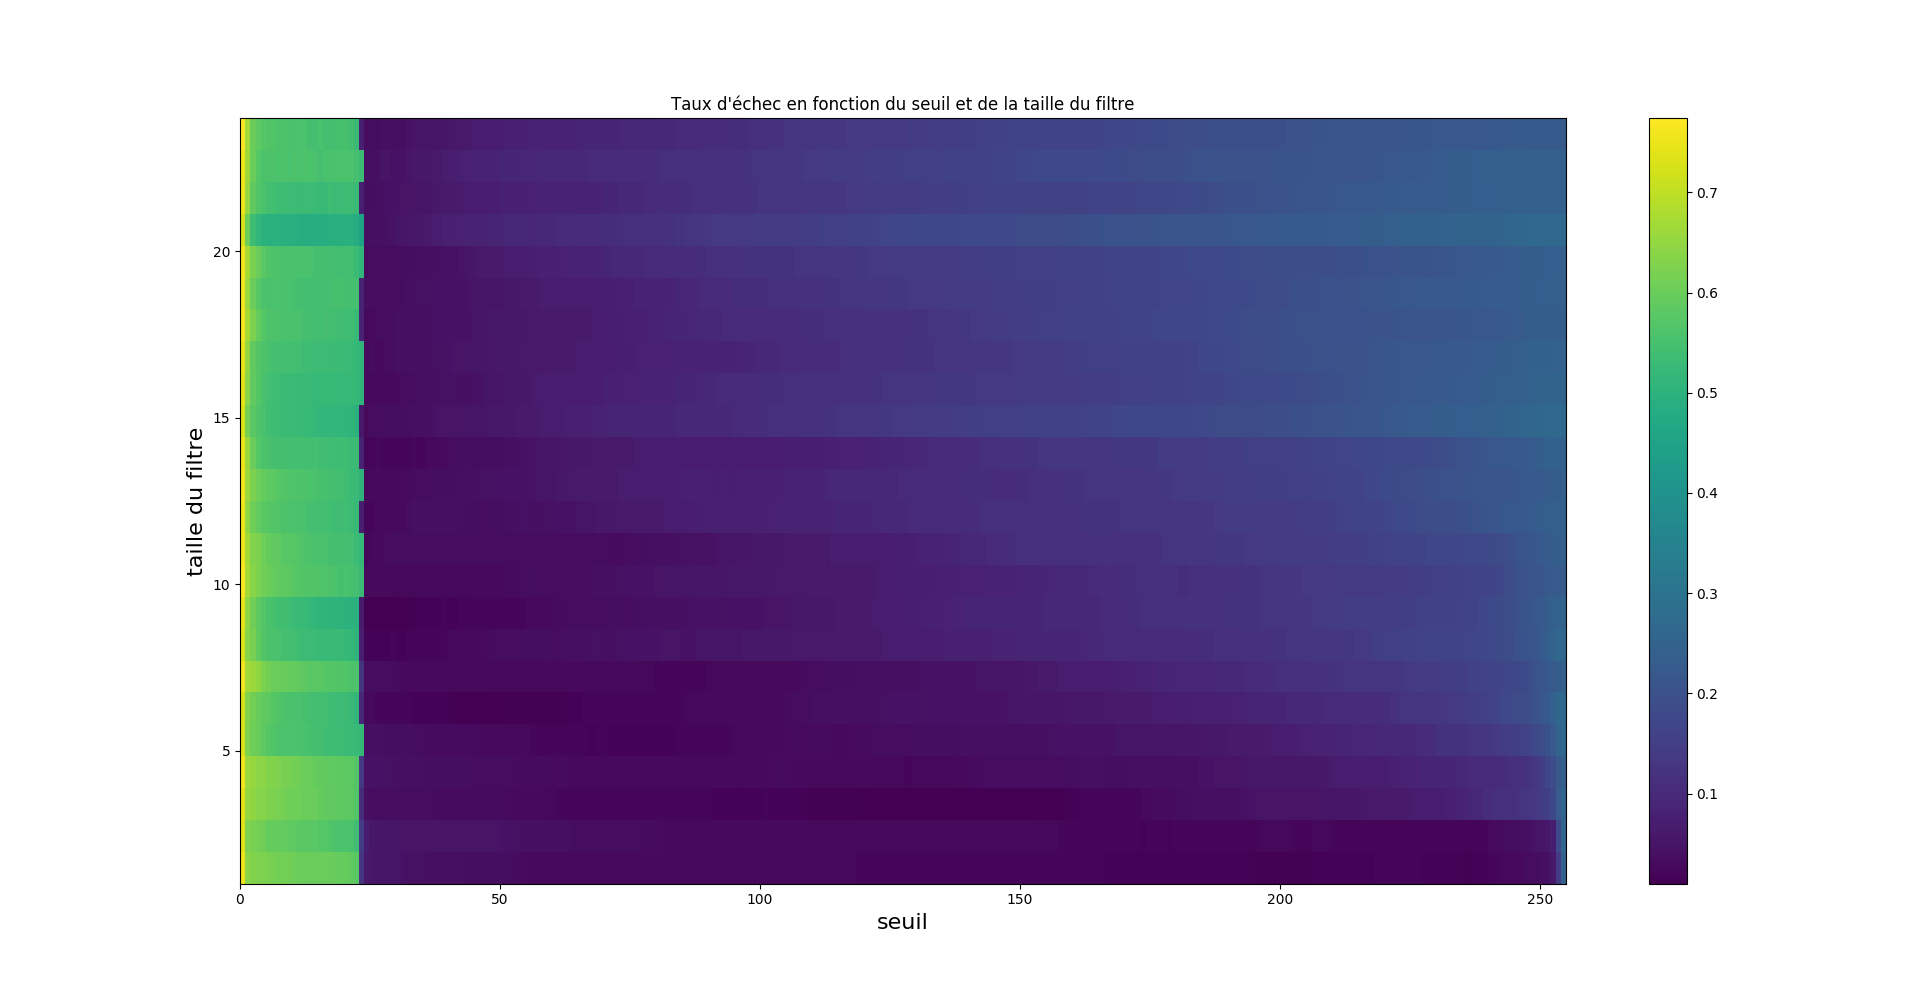
\includegraphics{filtre_vs_seuil.png}
\end{frame}


\end{document}
